\documentclass{article}
%\usepackage{url}
\usepackage{hyperref}
\usepackage{graphicx}

\begin{document}


\title{Resequencing against a sequence graph}

\author{Erik Garrison}

\maketitle

\begin{abstract}
Despite the availability of whole genome sequences from many individuals in many species, when examining a new genome we only use single reference haplotype as our basis for interpretation. As a result, our analyses are biased against the detection of any variation comprising significant differences from this reference haplotype. To resolve this issue, and also to expand resequencing approaches to organisms for which no single reference sequence has been (or can be) constructed, we propose the use of sequence graphs that simultaneously describe all known genomes. We first outline the basic model. Then, we describe its implementation in a reusable software library.
\end{abstract}

\section{Introduction}

Where genomes are small and sequences from different individuals can be reliably isolated, we can understand variation by assembling whole genomes and then comparing them via whole-genome comparison approaches \cite{mummer}.
However, as the genomes of organisms of interest (such as \emph{Homo sapiens}) are often large \cite{pmid11237011}, and the genomes of organisms we want to understand are often complex and difficult to completely assemble reliably using existing technology (for example, that of \emph{Plasmodium falciparum} still contains 80 gaps \cite{pfalciparum, pfalciparumweb}), standard practice involves the localization of short reads against a single high-quality reference system that is typically composed of a single haplotype per homologous region. Conceptually, this reference describes a single hypothetical individual, although in practice sequences from many individuals may be used to generate the assembly.

In \emph{resequencing}, we use alignments against a set of reference sequences (typically chromosomes or assembly contigs) to describe variation in a new sample. By linking new observations into a common reference system, resequencing provides a coherent approach to relate the genomes of individuals in an entire population. However, as this approach requires sufficient similarity between variant sequences in order to relate them, we may be unable to directly observe many kinds of variation, such as large insertions and deletions of sequence (indels) or even clusters of smaller variation (such as single nucleotide polymorphisms, SNPs). Indels, which contribute significantly to sequence diversity \cite{mills2010}, are particularly difficult, in that sequences derived from insertions relative to the reference sequence cannot be easily localized against the reference. This contributes significantly to the difficulty of genotyping transposable element insertion polymorphisms, which are still poorly-understood despite the efforts of large-scale sequencing projects \cite{stewart2011}. Similarly, copy-number variations, which influence large regions of the human genome, are difficult to genotype in new samples even when previously-known \cite{sudmant2010}.

Although these problems are more general than the specific resequencing informatics techniques that are applied, in all cases the basic problem is that cost of discovery of novel variation is equivalent to the cost of genotyping known variation in a new sample. However, this effort seems wasted, as most variation is shared, particularly in species with relatively small effective population sizes such as humans. Resources such as that produced by the 1000 Genomes Project now contain the vast majority (greater than $95\%$) of variation that we expect to find in a newly-sequenced human individual \cite{1000Gphase1}. If we could generate a reference system including this variation, we could reduce the cost of genotyping it in new samples. We now describe a basic model for such a system and the implementation of data formats and a software library designed to enable resequencing approaches to operate against this generalize reference system.

\section{Methods}

A traditional model to combine variation from many samples into one reference system is the multiple sequence alignment (\hyperref[fig:msa]{figure \ref{fig:msa}}). In this approach, sequences are encoded using an additional gap character, typically represented as ``-'', which indicates when one sequence in the multiple sequence alignment (MSA) has additional sequence where the one in which the gap is included does not. This mutually-gapped alignment has the desirable property that it fully-represents all of the sequences which were mutually aligned. This model has a dual representation as a partially-ordered graph in which homologous sequences are compressed into a single representation (\hyperref[fig:poa]{figure \ref{fig:poa}}). Generalizations of pairwise alignment \cite{gotoh1982} allow the alignment of new sequences directly to this structure in $O(NM)$ time, where $N$ is the length of the query and $M$ the sum of lengths of unique sequences in the partially-ordered sequence graph \cite{lee2002POA}.

While the POA representation of sequence variation in many samples is complete, the requirement of partial ordering limits its use to contexts where the complete synteny of a particular region can be established. A more general model for representing many sequences in the same context and allowing for cycles is the string graph, proposed by \cite{myers2005} and implemented efficiently by \cite{simpson2010}.

\section{Results}

\section{Discussion}

\bibliography{references}{}

\bibliographystyle{plain}

\begin{figure}
\centering
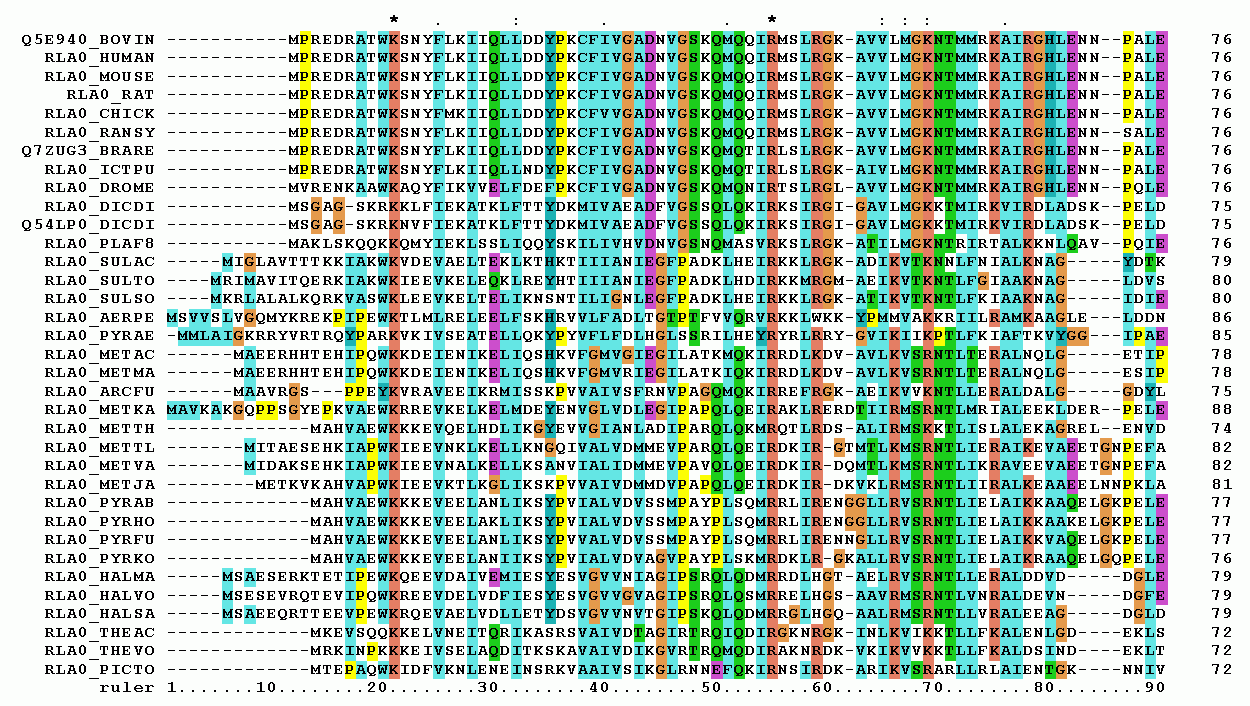
\includegraphics[width=1.0\textwidth]{figures/RPLP0_90_ClustalW_aln}
\caption{\label{fig:msa}
  First 90 positions of a protein multiple sequence alignment of instances of the acidic ribosomal protein P0 (L10E) from several organisms. Generated with ClustalX. Credit: Miguel Andrade \url{https://commons.wikimedia.org/wiki/File:RPLP0_90_ClustalW_aln.gif}. CC BY-SA 3.0.
}
\end{figure}

\begin{figure}
\centering
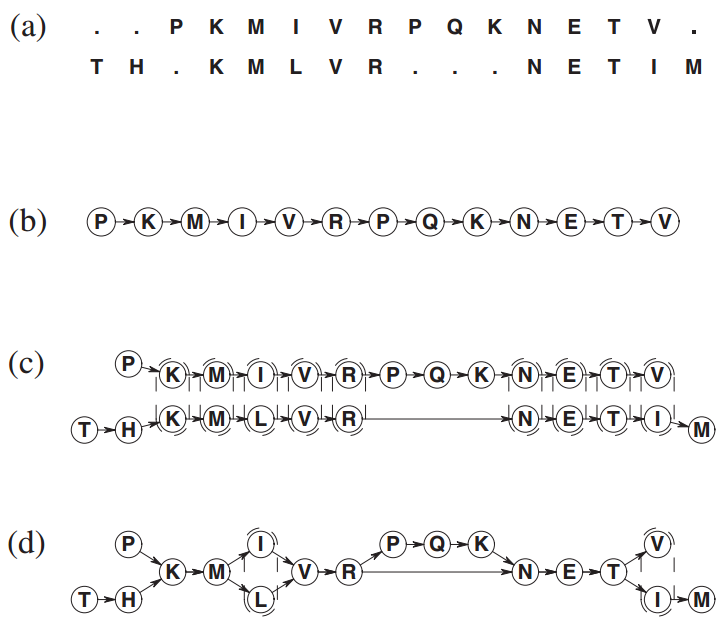
\includegraphics[width=0.8\textwidth]{figures/poamsa}
\caption{\label{fig:poa}
The relationship between a multiple sequence alignment (MSA) and a partially-ordered sequence graph (POA). (a) A gapped MSA representation for a pairwise protein alignment. (b) A single sequence in POA format. (c) The alignment of two sequences in POA format. (d) The POA representation of the original MSA. From \cite{lee2002POA}.
}
\end{figure}


\end{document}
